\newcommand\hii{\ion{H}{ii}}

\section{Comparison with observations}
\label{sec:comp-with-observ}


Placing various classes of objects on the \(R_{90}\)--\(R_c\) plane:
\begin{itemize}
\item LL arcs
\item runaway O stars
\item AGB stars
\end{itemize}

\subsection{Mid-infrared arcs around early-type stars}
\label{sec:mid-infrared-arcs}

\begin{figure*}
  \setlength\tabcolsep{0pt}
  \begin{tabular}{ll}
    (a)
    & (b) \\
    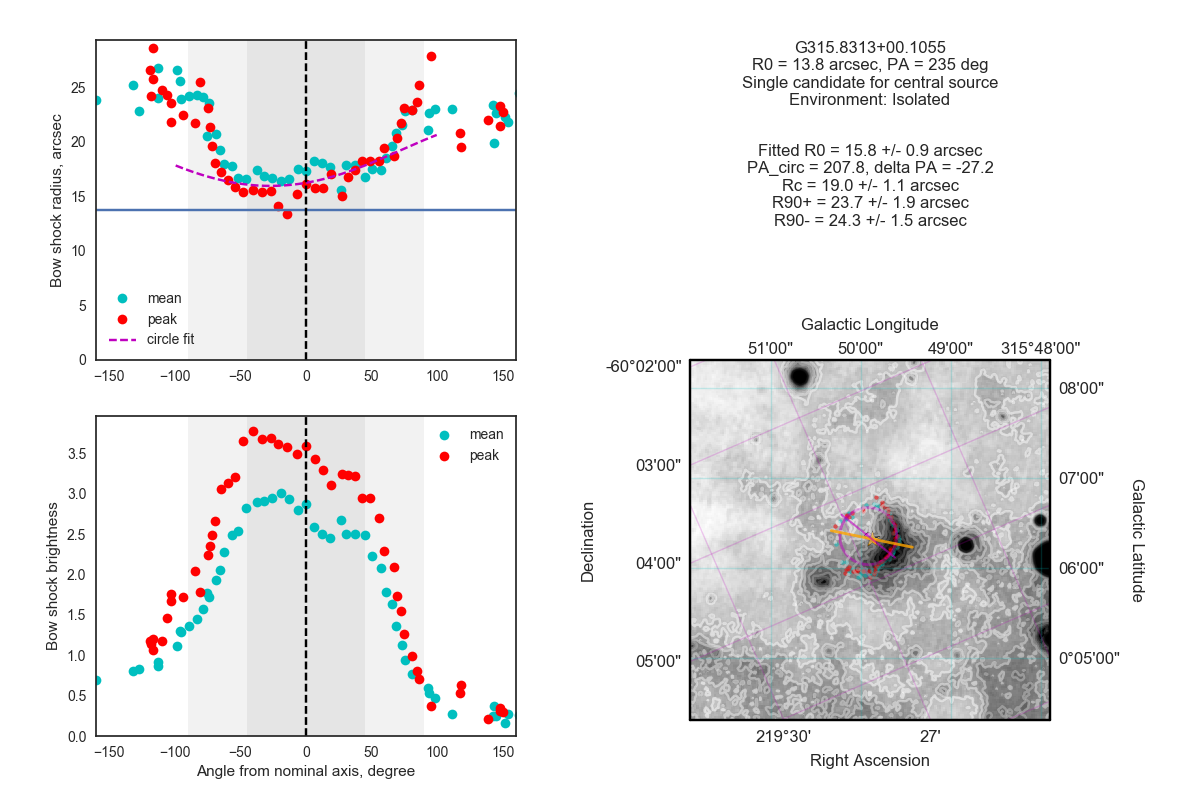
\includegraphics
    [width=0.5\linewidth, trim=20 15 30 10, clip]{figs/0510-3-star}
    & 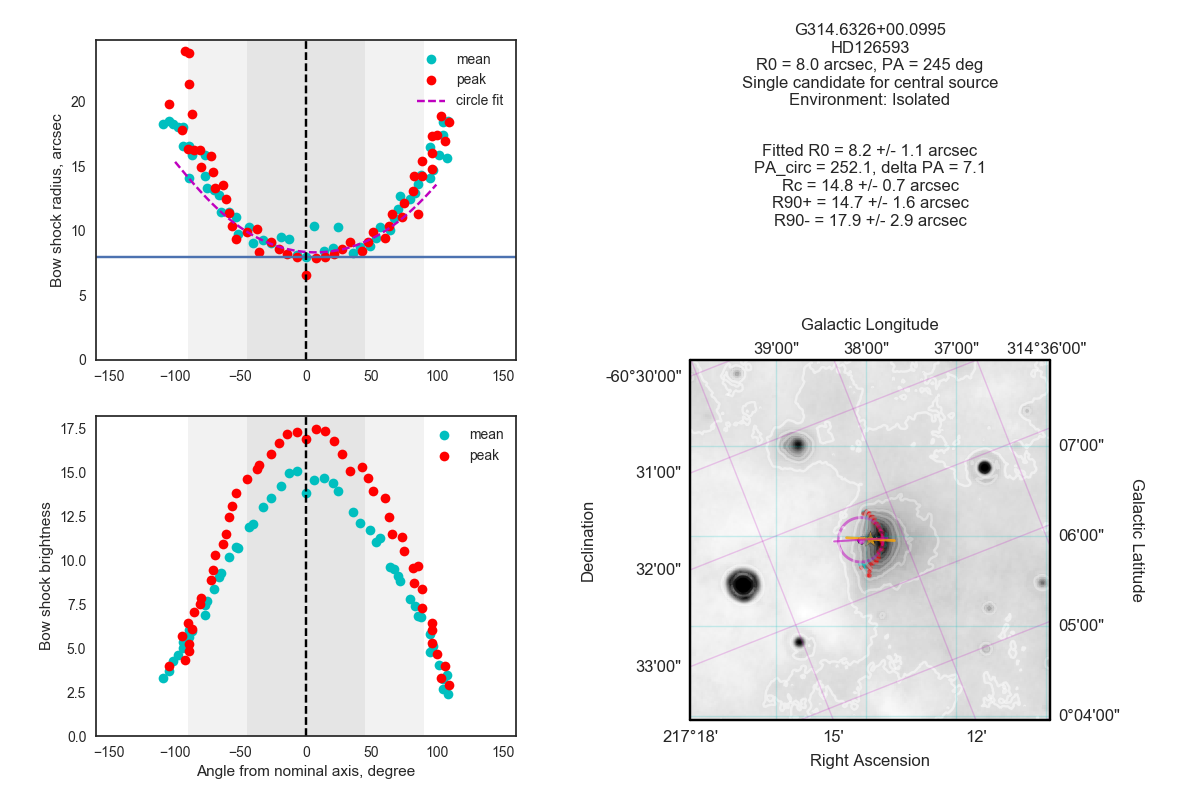
\includegraphics
      [width=0.5\linewidth, trim=20 15 30 10, clip]{figs/0506-4-star} \\
    (c)
    & (d) \\
    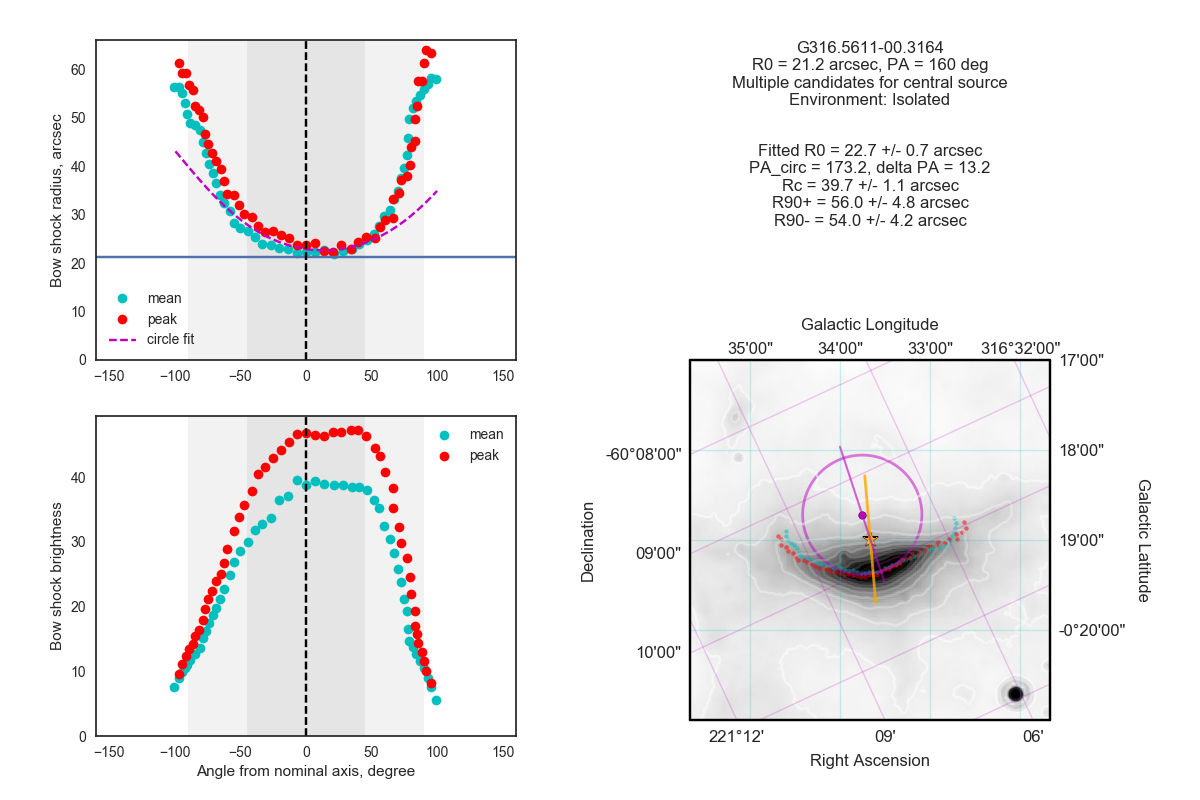
\includegraphics
    [width=0.5\linewidth, trim=20 15 30 10, clip]{figs/0517-5-star}
    & \multicolumn{1}{c}
      {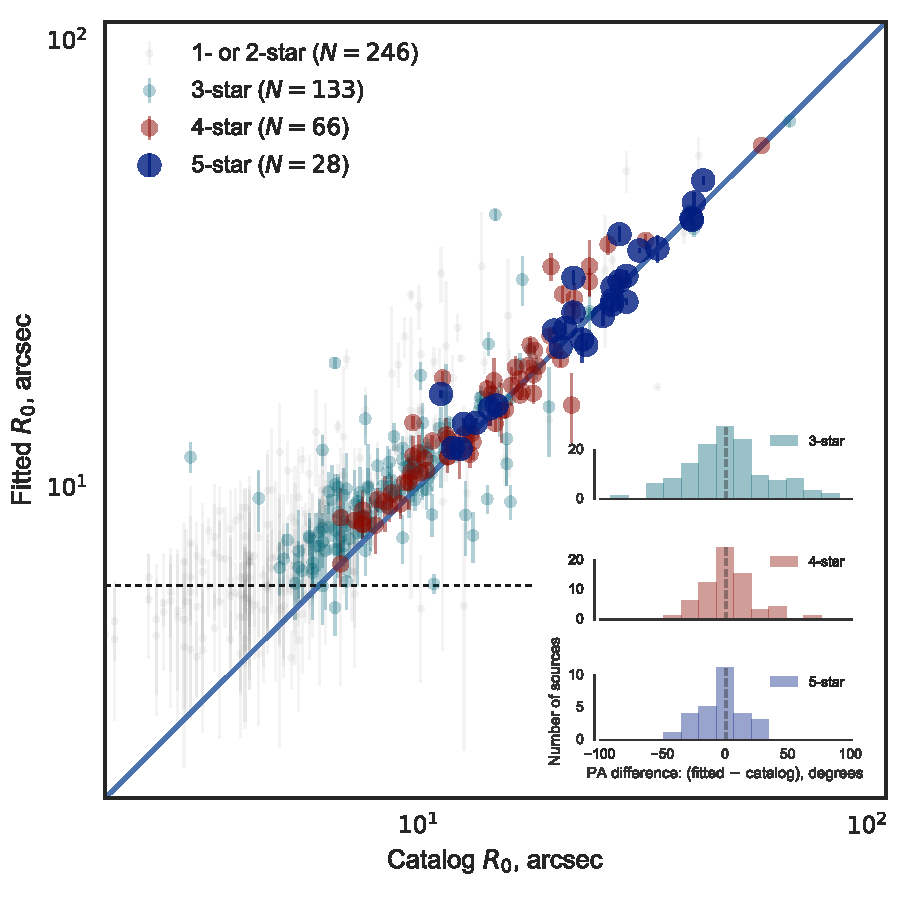
\includegraphics[width=0.35\linewidth, trim=20 20 20 20]
      {figs/mipsgal-r0-r0-plus-dPA-edited}}
  \end{tabular}
  \caption[]{Examples of typical fits to the bow shock shapes of
    MIPSGAL sources with different star ratings: (a) K510, 3-star
    rating; (b) K506, 4-star rating; (c) K517, 5-star rating.  Right
    panels of parts (a)--(c) show a 4\('\) square \SI{24}{\um} image,
    centered on each source.  Contours are ten linearly spaced levels
    between the median brightness of the entire image and the maximum
    brightness of the bow shock arc. Grids of galactic coordinates
    (light blue lines, parallel to the box sides) and equatorial
    coordinates (tilted magenta lines) are shown.  The stellar source
    and the bow shock axis, as determined by \citet{Kobulnicky:2016a}
    are indicated by an orange star and an orange line, respectively,
    where the line extends from \(-2 R_0\) to \(+2 R_0\).  The
    automatically traced arc shapes using the ``mean'' and ``peak''
    methods (see text) are shown by blue and red dots, respectively.
    The magenta circle shows the fit to the arc points within
    \(\pm 45^\circ\) of the nominal bowshock axis, with the magenta dot
    showing the center of curvature and the magenta line showing the
    fitted bow shock axis, which is the line passing through the
    source and the center of curvature.  Left panels of parts (a)--(c)
    show the radius measured from the source (upper panel) and
    brightness (lower panel) of the arc points, plotted as a function
    of angle \(\theta\) from the nominal bow shock axis, and with the same
    color coding as used on the image. Angular ranges of
    \(\theta = \pm 45\degr\) and \(\pm 90\degr\) are shown by gray shaded
    boxes In the upper panel, the \(R_0\) value tabulated by
    \citet{Kobulnicky:2016a} is shown by a horizontal blue line. (d)
    Comparison of the bow shock sizes (scatter plot) and position
    angles (inset histograms) determined from our fits with those
    tabulated by \citet{Kobulnicky:2016a} for the MIPSGAL sources.}
  \label{fig:mipsgal-examples}
\end{figure*}


The most extensive observational sample of stellar bow shock nebulae
to date is a catalog of 709 arcs \citep{Kobulnicky:2016a} detected in
mid-infrared surveys of the Galactic Plane by the \textit{Spitzer
  Space Telescope} (\textit{SST}, \citealp{Werner:2004a}) and
\textit{Wide-field Infrared Survey Explorer} (\textit{WISE},
\citealp{Wright:2010a}).  These sources are believed to be powered by
the winds of early-type stars, which are either moving supersonically
through the interstellar medium (runaway stars,
\citealp{Gvaramadze:2008a}), or are interacting with a local bulk
flow, such as the champagne flow from a nearby \hii{} region (weather
vanes, \citealp{Povich:2008a}).

In order to study the shapes of these bow shocks, we downloaded data
from the NASA/IPAC Infrared Science Archive archive\footnote{
  \url{http://irsa.ipac.caltech.edu/docs/program_interface/api_images.html}}
and extracted 4\arcmin{} square images in the \SI{24}{\um} bandpass of
the Multiband Imaging Photometer for \textit{Spitzer} (MIPS) centered
on each of the 471 \citet{Kobulnicky:2016a} sources that are covered
by the MIPSGAL \citep{Carey:2009a} survey, which includes most of the
sources with Galactic longitude within \(\pm 60\degr\) of the Galactic
center.

We developed a methodology for automatically tracing the arcs as follows:
\begin{enumerate}[1.]
\item Calculate arrays of celestial coordinates, \(C\), for each pixel
  of the image.
\item Using the central source coordinates, \(C_0\) and nominal
  bowshock radius, \(R_0\) from \citet{Kobulnicky:2016a}, construct a
  pixel mask that includes only those pixels with separations from the
  source that satisfy \(\frac12 R_0 \le |C - C_0| \le 3 R_0\).  This mask
  will be used for all subsequent operations, which serves to help
  avoid confusion from the star itself and other bright sources in the
  field of view.
\item Define a ``step-back'' point, \(C_1\), which is located at a
  separation \(2 R_0\) from the source, but in the opposite direction
  from the apex of the bow shock. That is, along a position angle
  180\degr{} from the nominal position angle, \(\text{PA}_0\), of the
  bow shock axis.  This point is at one end of the orange line shown
  superimposed on the bow shock images in
  Figure~\ref{fig:mipsgal-examples}.
\item Looping over a grid of 50 position angles, \(\text{PA}_k\),
  within \(\pm 60\degr\) of \(\text{PA}_0\), estimate the location of
  the arc along rays cast from the step-back point, using two
  different methods:
  \begin{enumerate}[(a)]
  \item The pixel with the peak brightness, with coordinates
    \(C_{k,\text{peak}}\) (red dots in
    Fig.~\ref{fig:mipsgal-examples}).
  \item The mean brightness-weighted separation from \(C_1\), with
    coordinates \(C_{k,\text{mean}}\) (light blue dots in
    Fig.~\ref{fig:mipsgal-examples}).
  \end{enumerate}
  For each \(\text{PA}_k\) in the grid, the calculation is performed
  over only those pixels that satisfy
  \(|\text{PA}(C, C_1) - \text{PA}_k| < \frac12 \delta\theta\), where
  \(\delta\theta = 120/50 = 2.4\degr\), which defines a thin radial wedge from
  \(C_1\).  The results are shown as red and blue dots superimposed
  on the images in Figure~\ref{fig:mipsgal-examples}. Each of the two
  methods, ``peak'' and ``mean'', works better in some objects and
  worse in others (according to the subjective judgment of
  ``correctly'' tracing the bow shock shape).  We therefore take the
  average by amalgamating all the \(C_{k,\text{peak}}\) and
  \(C_{k,\text{mean}}\) points into a single set, \(C_{k}\), for
  the following steps.
\item For each of the points \(C_{k}\), determine the radial
  separation from the central source, \(R_k = |C_k - C_0|\) and the
  angle from the bow shock axis about the central source
  \(\theta_k = \text{PA}(C_k, C_0) - \text{PA}_0\).  These are plotted in
  the upper left panels of Figure~\ref{fig:mipsgal-examples}.  Note
  that, even though the rays are cast from the step-back point \(C_1\)
  within \(\pm 60\degr\) of \(\text{PA}_0\), the angles \(\theta_k\) are
  measured from the source, \(C_0\), which is closer to the bow shock
  than \(C_1\) and therefore \(|\theta_k|\) can be much larger than
  \(60\degr\).
\item Make our own estimate of the axial size, \(R_0\), of the bow
  shock by calculating the mean and standard deviation of \(R_k\) over
  all points \(C_k\) with \(|\theta_k| \le 10\degr\).  Note that this is
  distinct from the nominal value of \(R_0\) given in the
  \citet{Kobulnicky:2016a} catalog, which was ``measured by eye''.
\item Estimate the radius of curvature, \(R_c\), by fitting a circle
  to all those points within \(\pm 45\degr\) of the nominal axis
  (\(|\theta_k| < 45\degr\)), but after excluding any point with
  \(R_k < \frac12 R_m\) or \(R_k > 2 R_m\), where \(R_m\) is the median
  \(R_k\) for \(|\theta_k| < 45\degr\).
\item Determine two separate estimates, \(R_{90+}\) and \(R_{90-}\),
  of the perpendicular radius, \(R_{90}\), by taking the mean and
  standard deviation of \(R_k\) over all points \(C_k\) with
  \(|\theta_k - 90\degr| \le 10\degr\) for \(R_{90+}\), and with
  \(|\theta_k + 90\degr| \le 10\degr\) for \(R_{90-}\).
\end{enumerate}

After these automatic steps, we subjectively evaluate the results by giving a star rating to each source:

\paragraph*{0 stars} The fitting algorithm failed for some reason. 

\paragraph*{1 star} The fit was formally successful, but the results
for \(R_c\) or \(R_{90}\) are far removed from what a human would
predict by looking at the image.  For example, in the smallest
bowshocks, which are only marginally resolved by Spitzer's 6\arcsec{}
beam, the dispersion in \(R_k\) can be a significant fraction of
\(R_0\), in which case our algorithm tends to erroneously favor
\(R_c < R_0\).

\paragraph*{2 stars} The fit results are not totally outlandish, but
nonetheless some problem is apparent that casts doubt on their
reliability.  For example, a double-shell structure to the bow shock
that leads to large differences between the ``peak'' and ``mean''
methods, or point sources near to the bow shock that interfere with
the tracing procedure.
  
\paragraph*{3 stars} A good fit, but where the dispersion in \(R_k\)
and/or the asymmetry in the bow shock reduces the precision in the
determination of \(R_c\) and \(R_{90}\), giving subjectively estimated
uncertainties around the 20\% level.  An example of a 3-star fit is
shown in Figure~\ref{fig:mipsgal-examples}a.

\paragraph*{4 stars} A high quality fit, with subjectively estimated
uncertainties in \(R_c\) and \(R_{90}\) around the 10\% level. An
example of a 4-star fit is shown in
Figure~\ref{fig:mipsgal-examples}b.

\paragraph*{5 stars} The highest-quality fit, usually corresponding to
large, sharply defined bow shocks, whose shape is determined with high
precision. An example of a 5-star fit is shown in
Figure~\ref{fig:mipsgal-examples}c.

\bigskip
%
Figure~\ref{fig:mipsgal-examples}d compares the bow shock size,
\(R_0\), determined by our fits (vertical axis) with the corresponding
value given in the \citet{Kobulnicky:2016a} catalog (horizontal axis).
For most sources with 3-star or higher rating, the two estimates agree
to within \(\pm 20\%\), but there are a small number of sources with a
discrepancy of more than a factor of two.  In all cases that we
checked, we believe that our estimates of \(R_0\) are more accurate
than those in the catalog.  It is apparent that the star ratings are
correlated with the bow shock size, with larger bow shocks tending to
receive higher ratings, although there is considerable overlap.  In
particular, most of the 1- and 2-star sources are close to the
resolution limit of the MIPSGAL \SI{24}{\um} images (\(6\arcsec\),
indicated by the dotted horizontal line in te figure).

In the following analysis, only those sources with a 3-star or higher
rating are used.  These comprise approximately half (227 out of 471)
of all the MIPSGAL arc sources.  In some cases of poor and failed
fits, there is nothing apparently ``wrong'' with the source itself,
and it is likely that minor tweaks to the methodology would improve
matters, but we have elected not to do so, in order to maintain a
uniform methodology across all sources.

The inset of Figure~\ref{fig:mipsgal-examples}d shows histograms of the difference between the position angle determined by our fits and that listed in \citet{Kobulnicky:2016a}.  



\begin{figure*}
  \centering
  \begin{tabular}{ll}
    (a) & (b) \\
    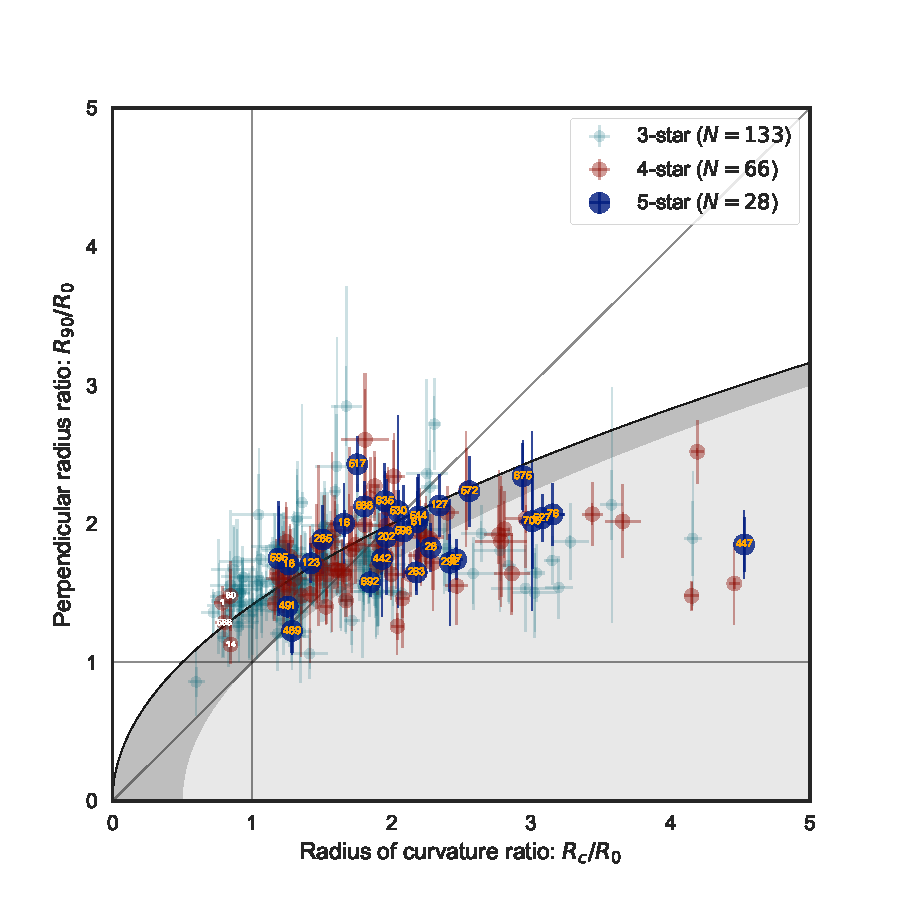
\includegraphics[width=0.45\textwidth]{figs/mipsgal-Rc-R90-zoom} &
    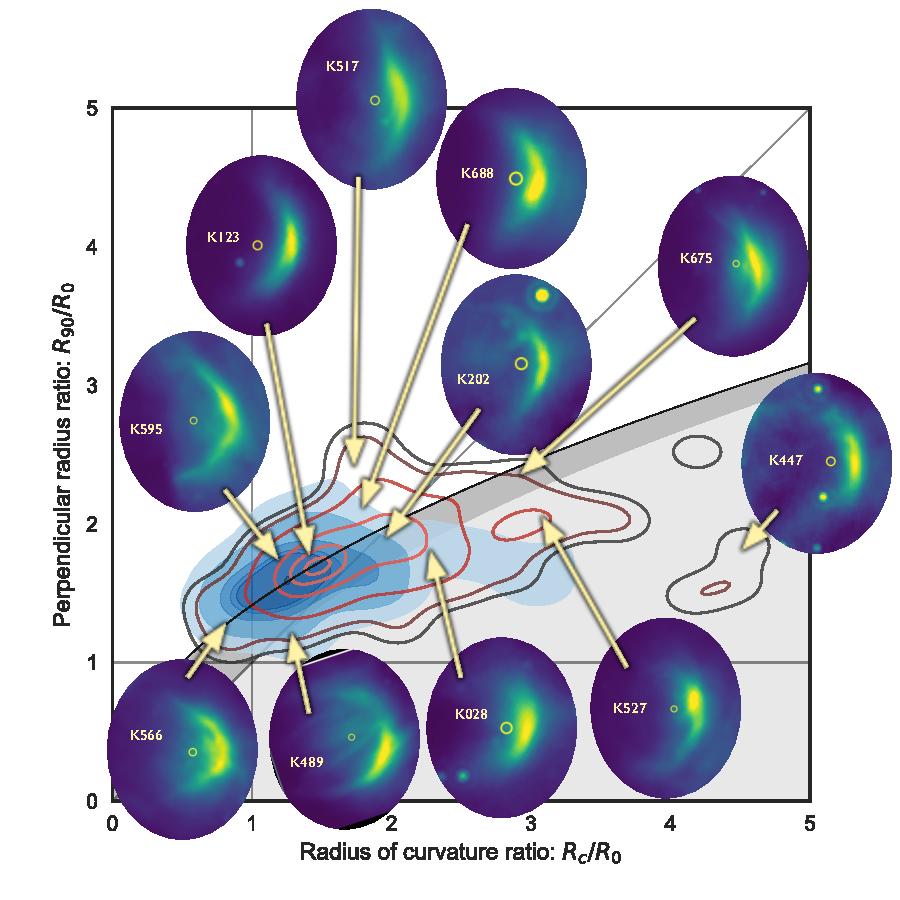
\includegraphics[width=0.45\textwidth]{figs/mipsgal-Rc-R90-thumbnails} 
  \end{tabular}
  \caption[]{MIPSGAL sources on the bow shock shape diagnostic
    diagram.  (a) Individual sources.  (b) Kernel density estimate of
    the distribution.}
  \label{fig:mipsgal-shapes}
\end{figure*}


\begin{figure*}
  \centering
  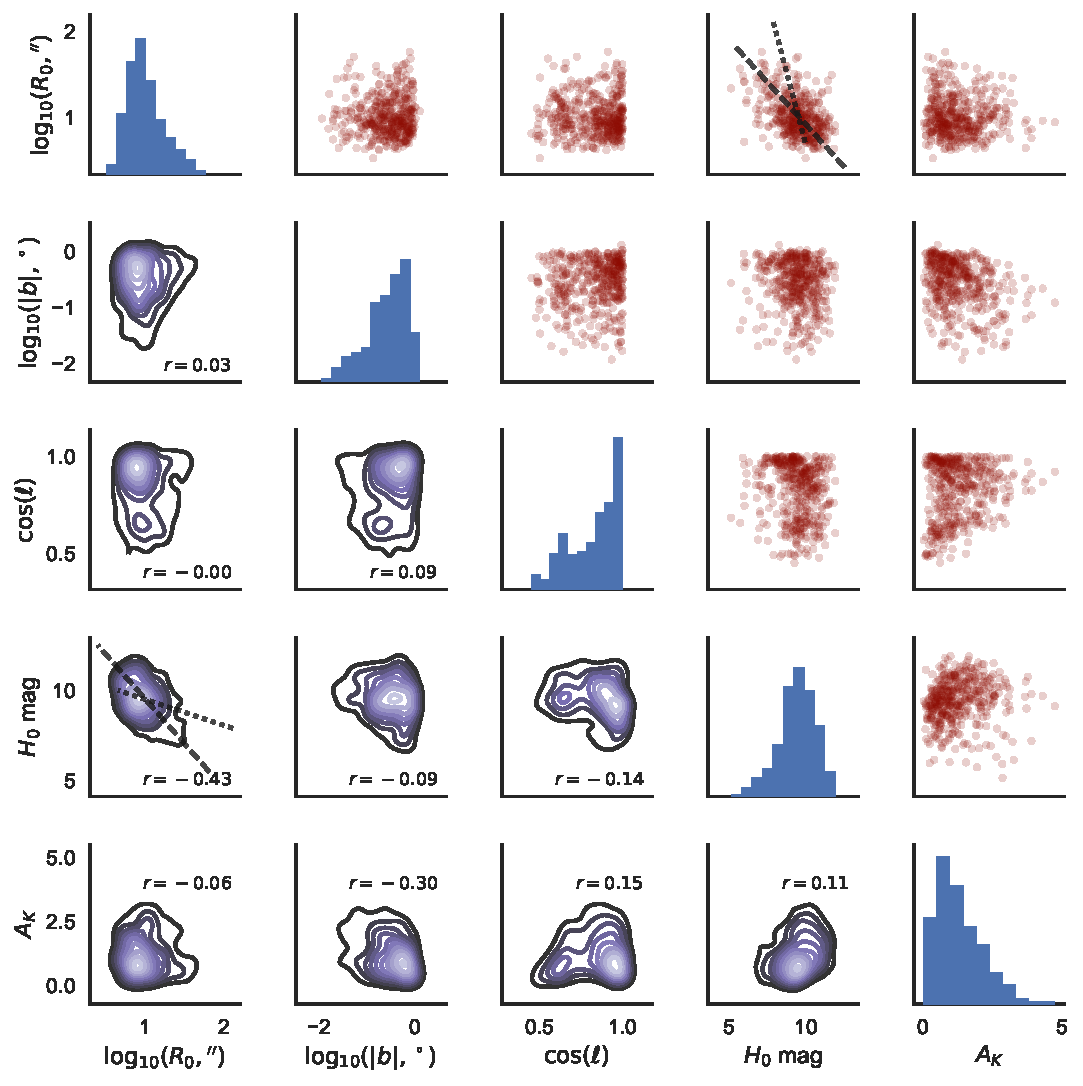
\includegraphics[width=\textwidth]{figs/mipsgal-pairplot}
  \caption[]{Correlations between non-shape parameters of MIPSGAL sources.}
  \label{fig:mipsgal-pairplot}
\end{figure*}

\begin{figure*}
  \centering
  \begin{tabular}{ll}
    (a) & (b) \\
    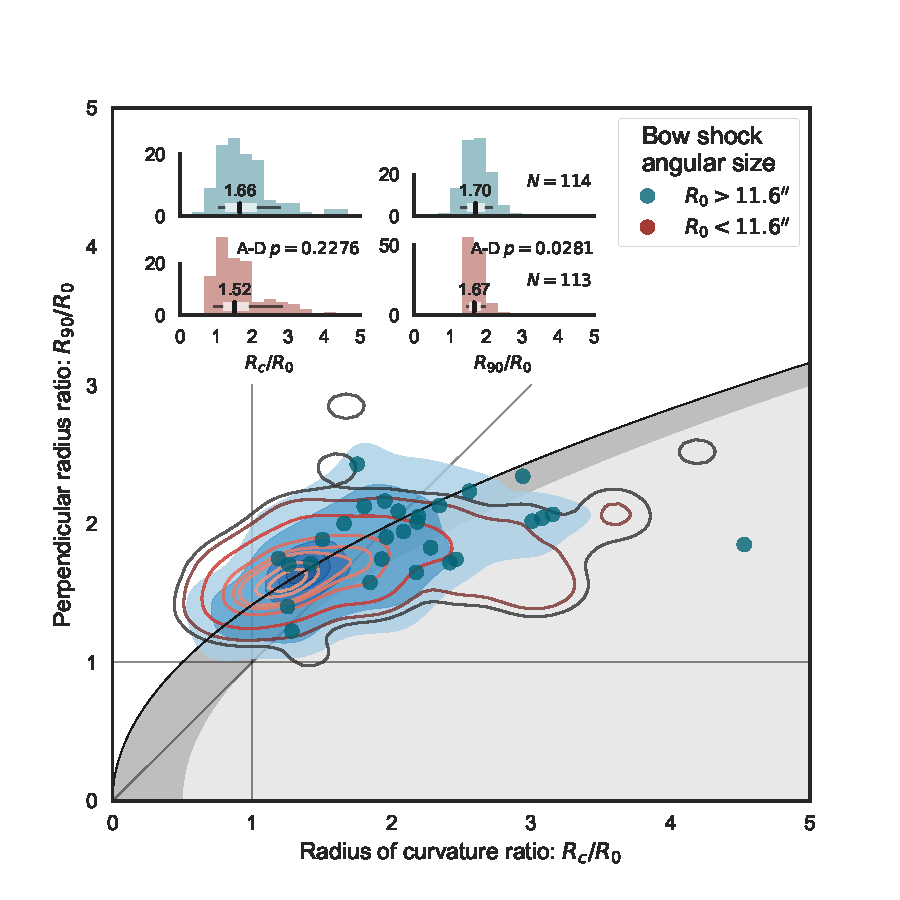
\includegraphics[width=0.45\textwidth]{figs/mipsgal-Rc-R90-R0} &
    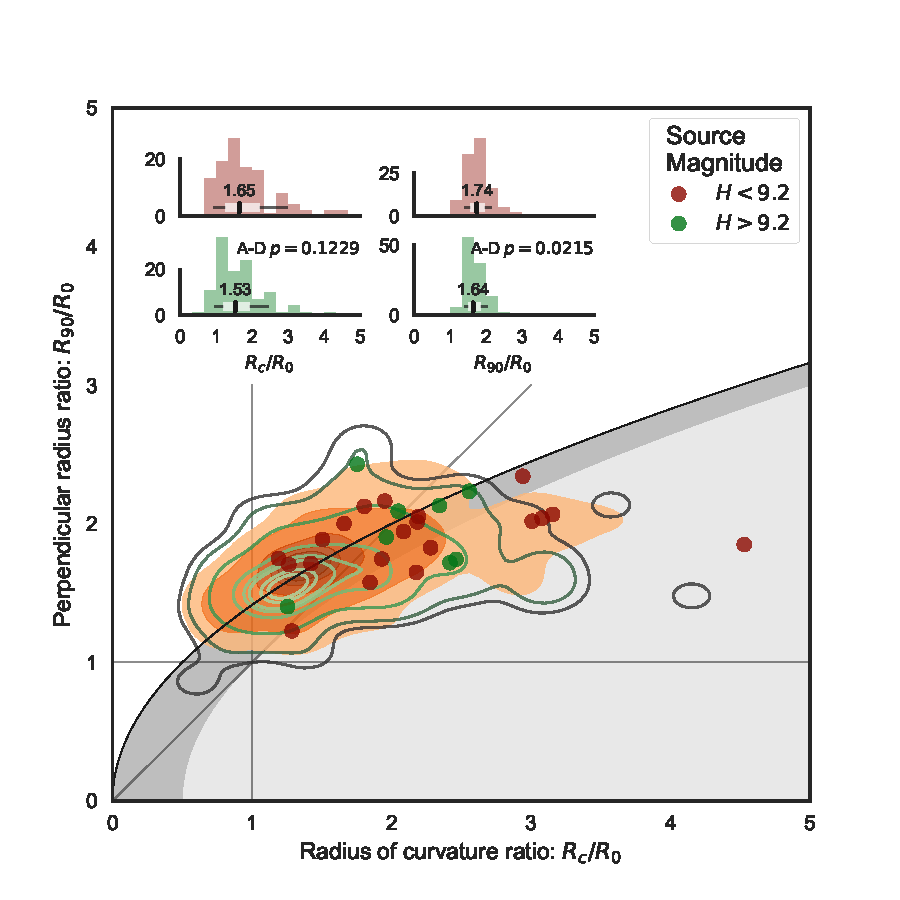
\includegraphics[width=0.45\textwidth]{figs/mipsgal-Rc-R90-Mag} 
  \end{tabular}
  \caption[]{Comparison between the distribution of bowshock shapes
    when the sources are divided into two sub-samples according to the
    value of another parameter. (a)~Bow shock angular size, \(R_0\).
    (b)~Extinction-corrected \(H\)-band magnitude of the stellar
    source.}
  \label{fig:mipsgal-correlated}
\end{figure*}

\begin{figure*}
  \centering
  \begin{tabular}{ll}
    (a) & (b) \\
    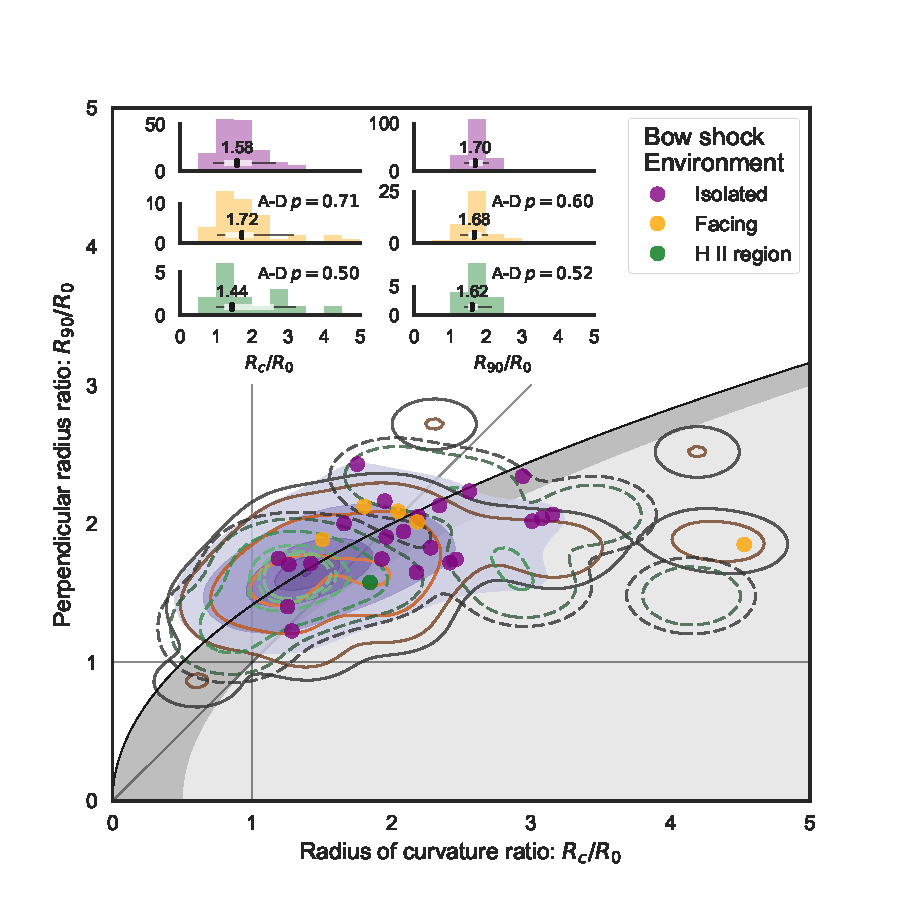
\includegraphics[width=0.45\textwidth]{figs/mipsgal-Rc-R90-environment} &
    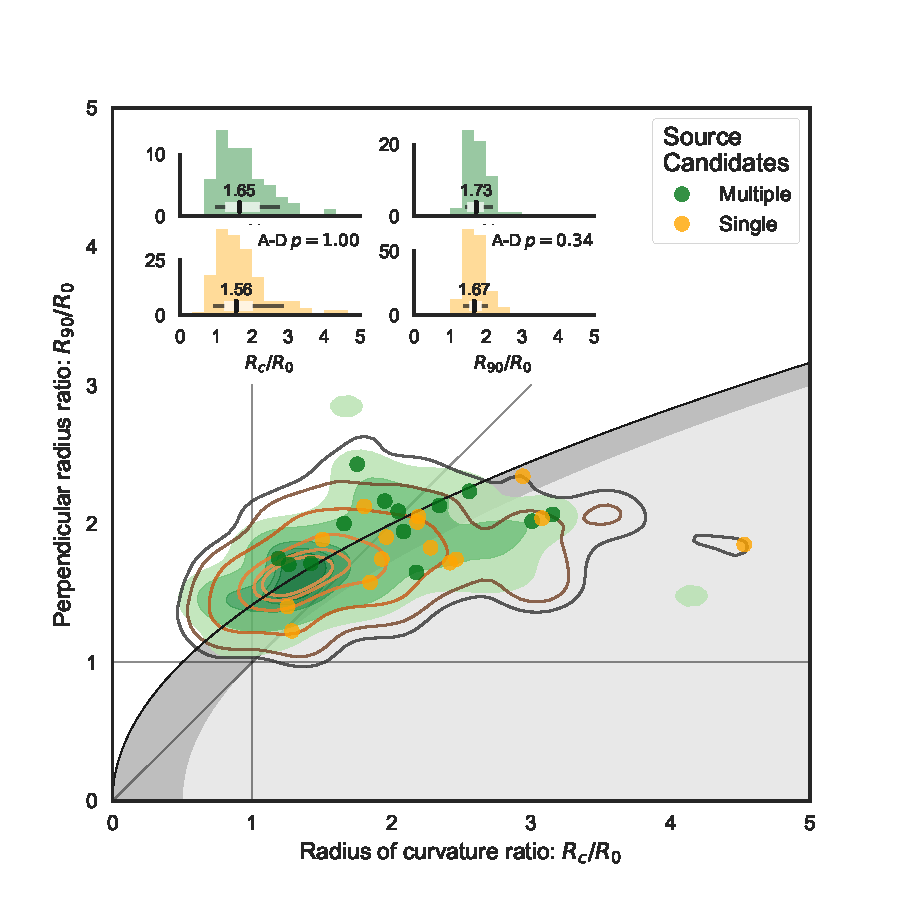
\includegraphics[width=0.45\textwidth]{figs/mipsgal-Rc-R90-candidates} 
  \end{tabular}
  \caption[]{Lack of significant correlation of bow shock shape with
    (a) environment, and (b) uncertainty in stellar source
    identification.}
  \label{fig:mipsgal-uncorrelated}
\end{figure*}


\subsection{Far-infrared arcs around late-type stars}
\label{sec:far-infrared-arcs}

\begin{figure}
  \centering
  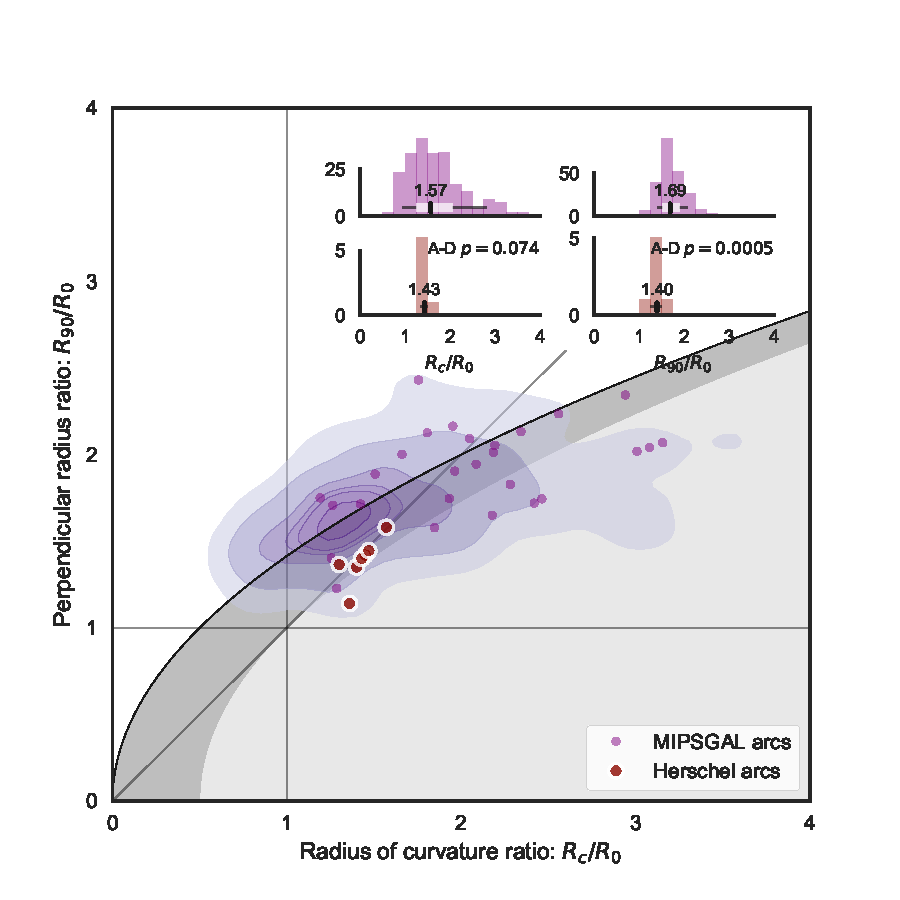
\includegraphics[width=\linewidth]{figs/mipsgal-Rc-R90-vs-Herschel}
  \caption[]{Comparison of RSG/AGB arcs with OB star arcs.}
  \label{fig:herschel-compare-mipsgal}
\end{figure}



\subsection{Stationary emission line arcs in M42}
\label{sec:stat-emiss-line}

\begin{figure*}
  \centering
  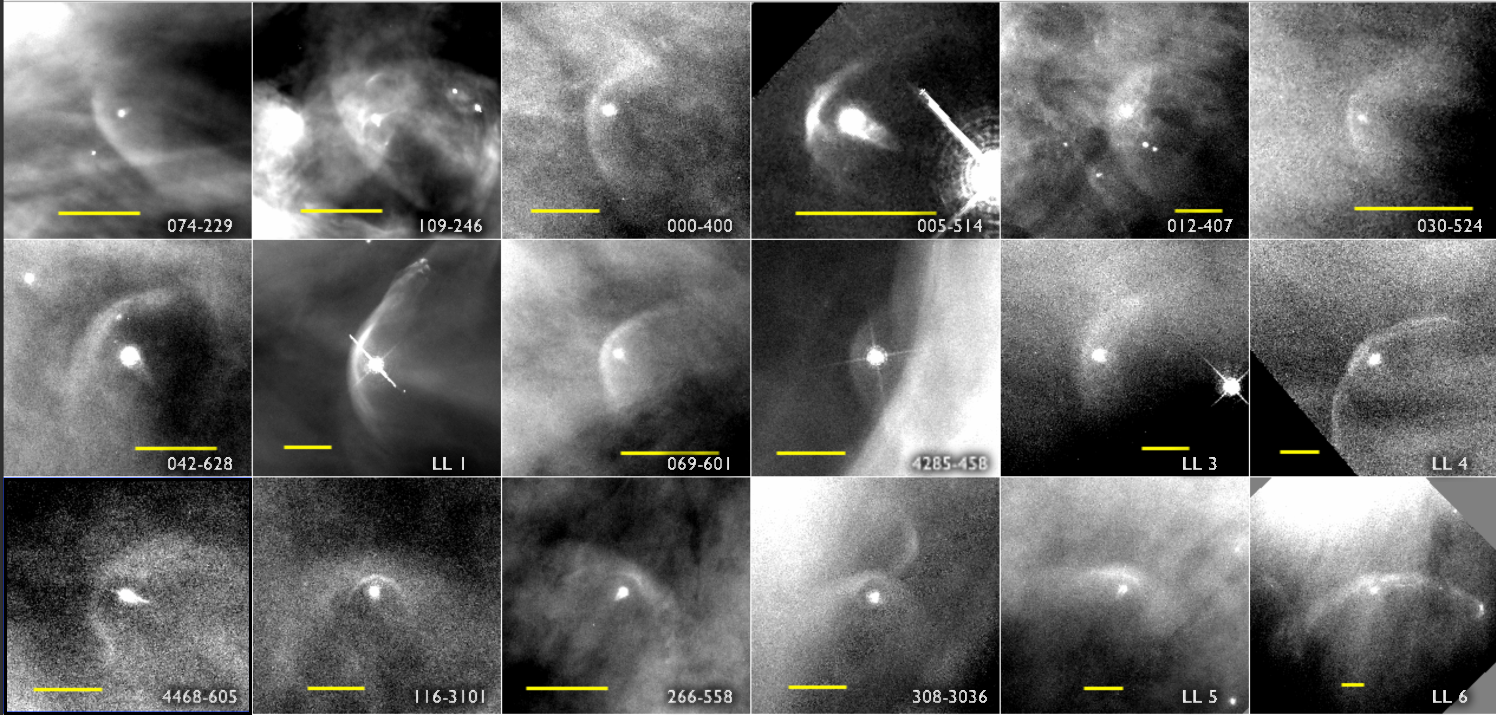
\includegraphics[width=\textwidth]{figs/annotated-ll-arcs}
  \caption[]{Stationary bow shock arcs in the Orion Nebula.}
  \label{fig:ll-arcs}
\end{figure*}

\begin{figure}
  \centering
  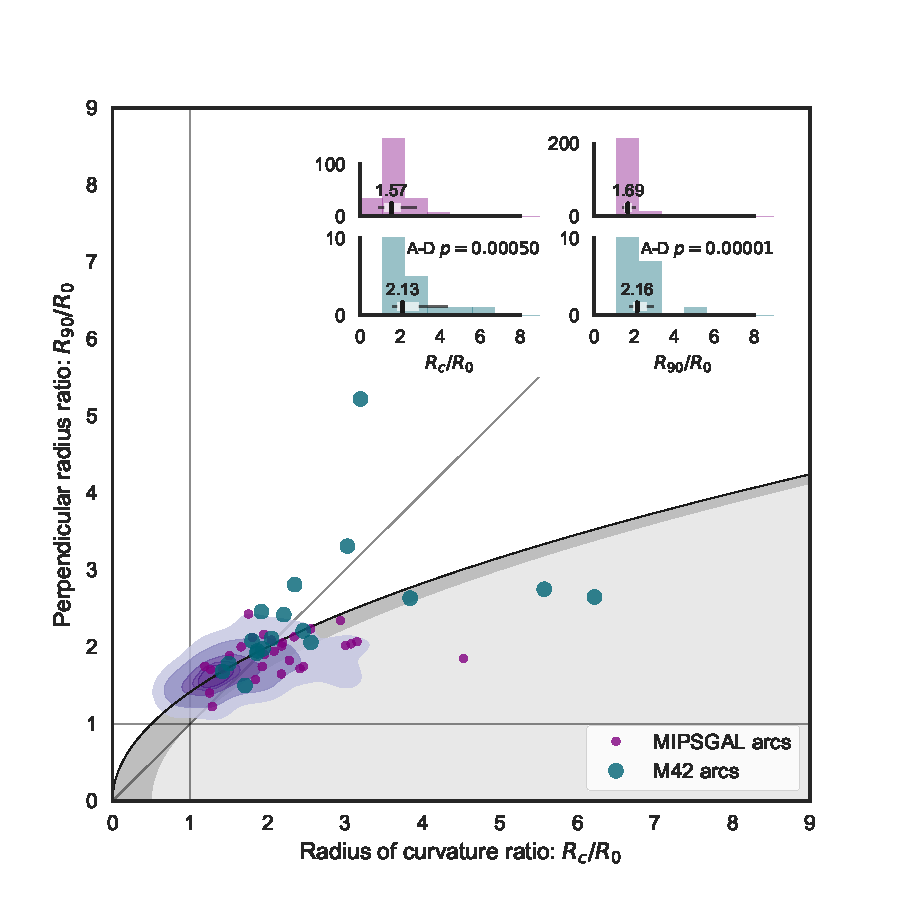
\includegraphics[width=\linewidth]{figs/mipsgal-Rc-R90-vs-Orion}
  \caption[]{Comparison of Orion with OB stars.}
  \label{fig:ll-compare-mipsgal}
\end{figure}




%%% Local Variables:
%%% mode: latex
%%% TeX-master: "quadrics-bowshock.tex"
%%% End:
